\documentclass[12pt]{article}
\usepackage[utf8]{inputenc}
\usepackage{amsmath,amsfonts,amssymb}
\usepackage{graphicx}
\usepackage{makeidx}
\usepackage{graphicx}
\usepackage{lmodern}
\usepackage{multicol}
\usepackage{booktabs}
\usepackage{fancyhdr}
\usepackage{hyperref}
\usepackage[usenames]{color}


\usepackage{Sweave}
\begin{document}
\Sconcordance{concordance:template_matching.tex:template_matching.Rnw:%
1 14 1 1 0 53 1 1 2 1 0 12 1 3 0 1 2 2 1 1 4 3 0 1 19 20 0 1 2 2 1 1 2 %
1 0 3 1 1 22 24 0 1 2 2 1 1 2 5 0 1 2 3 1 1 2 1 0 1 1 5 0 1 2 6 0 1 2 7 %
0 1 2 2 1 1 2 5 0 1 2 6 1 1 2 5 0 1 2 2 1 1 2 1 0 1 1 5 0 1 2 6 0 1 2 7 %
0 1 2 1 1 1 2 5 0 1 2 5 1 1 2 5 0 1 2 2 1 1 2 1 0 1 1 5 0 1 2 6 0 1 2 7 %
0 1 2 1 1 1 2 5 0 1 2 4 1 1 2 5 0 1 2 2 1 1 2 1 0 1 1 5 0 1 2 6 0 1 2 7 %
0 1 2 1 1 1 2 5 0 1 2 4 1 1 2 1 0 3 1 3 0 1 2 2 1 1 2 5 0 1 2 3 1 1 2 1 %
0 1 1 5 0 1 2 6 0 1 2 7 0 1 2 2 1 1 2 5 0 1 2 6 1 1 2 5 0 1 2 2 1 1 2 1 %
0 1 1 5 0 1 2 6 0 1 2 7 0 1 2 1 1 1 2 5 0 1 2 5 1 1 2 5 0 1 2 2 1 1 2 1 %
0 1 1 5 0 1 2 6 0 1 2 7 0 1 2 1 1 1 2 5 0 1 2 4 1 1 2 5 0 1 2 2 1 1 2 1 %
0 1 1 5 0 1 2 6 0 1 2 7 0 1 2 1 1 1 2 5 0 1 2 17 1}

\pagestyle{fancy}
\fancyhf{}
\renewcommand{\headrulewidth}{0.4pt}
\fancyfoot[C]{\thepage}
\renewcommand{\footrulewidth}{0.4pt}
\fancyfoot[C]{\thepage}
\title{\LARGE \bf
 Exercício  2 - Template Matching}
\author{ Rodrigo Machado Fonseca - 2017002253}
\thispagestyle{fancy}
\fancyhead[C]{Introdução ao Reconhecimento de Padrões - UFMG \\ Belo Horizonte - \today}
\maketitle
\thispagestyle{fancy}

%%%%%%%%%%%%%%%%%%%%%%%%%%%%%%%%%%%%%%%%%%%%%%%%%%%%%%%%%%%%%%%%%%%%%%%%%%%%%%%%%%%%%%%%%
\section{Introdução}
  \par Neste trabalho utlizaremos o algoritmo \textit{Template Matching} com o intuito de encontrar as placas 1 e 2 (figuras \ref{1} e \ref{2}) na figura geral (figura \ref{3}).
  
\section{Template Matching}
  \par O algoritmo Template Matching refere-se ao processamento de imagem em que encontramos modelos semelhantes em uma imagem de origem, fornecendo um modelo de base para comparação. O processo de correspondência do modelo é feito comparando cada um dos valores de pixel da imagem de origem, um de cada vez, com a imagem do modelo. A saída seria uma matriz de valores de similaridade em comparação com a imagem do modelo.
  
  \par A comparação do algoritmo pode ser feita com uma métrica de distância. Neste estudo utilizaremos a métrica de Minkowsky:
  \begin{equation}
    \delta_{mink}(x_i, x_j) = (\sum_{k=1}^n |x_{ik}-x_{jk}|^p)^{\frac{1}{p}}
    \label{mink}
  \end{equation}
  \par Na equação \ref{mink} podemos variar o valor de \textit{p} e teremos valores diferentes para o mesmo conjunto de pontos. Para os valores de $p=1$ e $p=2$ a fórmula fica equivalente a distância de Manhattan e a distância Euclidiana.
  
\section{Metodologia}
  \par Inicialmente, vamos carregar as imagens e transformá-las em escala de cinzas. O motivo disso é que, para figuras coloridas, cada pixel carrega três valores, que representam os valores de RGB, enquanto que em escala de cinzas o pixel só carregará um único valor. Assim, ao passá-los para escala de cinzas, limitamos o nosso problema a um único cálculo de distância por pixel.
  
  \begin{figure}[h]
   \centering
   
\includegraphics[width=0.4\linewidth]{placa_1.jpg}
   \caption{Placa 1}
   \label{1}
  \end{figure}
  
  \begin{figure}[h]
   \centering
   
\includegraphics[width=0.4\linewidth]{placa_2.jpg}
   \caption{Placa 2}
   \label{2}
  \end{figure}
  
  \begin{figure}[h]
   \centering
   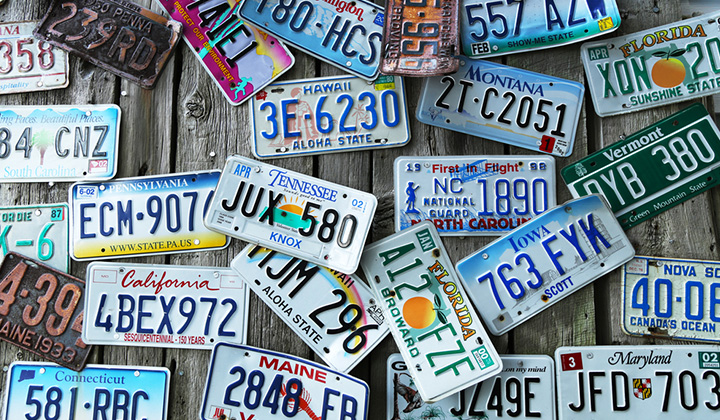
\includegraphics[width=0.7\linewidth]{placas.jpg}
   \caption{Figura geral}
   \label{3}
  \end{figure}

\begin{Schunk}
\begin{Sinput}
> rm(list=ls())
> library('jpeg')
> rotate <- function(x) t(apply(x, 2, rev))
> cor <- rev(gray(50:1/50))
> placa_1 <- readJPEG('placa_1.jpg', native = FALSE)
> image(rotate(placa_1[,,2]), col=cor)
> p1 <- rotate(placa_1[,,2])
> placa_2 <- readJPEG('placa_2.jpg', native = FALSE)
> image(rotate(placa_2[,,2]), col=cor)
> p2 <- rotate(placa_2[,,2])
> placas <- readJPEG('placas.jpg', native = FALSE)
> image(rotate(placas[,,2]), col=cor)
> Im <-rotate(placas[,,2])
\end{Sinput}
\end{Schunk}

  \par Após a transformação em escala de cinza, para aplicarmos o Template Macthing basta aplicarmos uma máscara do tamanho de cada placa no conjunto com todas as placas. Essa máscara irá aplicar a distância de Minkowsky. 

\begin{Schunk}
\begin{Sinput}
> minkowsky <-function(p, x1, x2){
+   return((sum(abs(x1-x2)^p)^(1/p)))
+ }
> find_board <- function(p, p1, Im){
+   nc <- (dim(Im)[2] - dim(p1)[2])
+   nl <- (dim(Im)[1] - dim(p1)[1])
+   d <- matrix(0, nl, nc)
+   min_dist <- matrix(nrow = length(p), ncol =1)
+   d_list <- list()
+   for(i in p){
+     for(l in 1:nl){
+       for(c in 1:nc){
+         d[l,c] <- minkowsky(i, Im[l:(l+dim(p1)[1]-1), 
+                                   c:(c+dim(p1)[2]-1)], p1)
+       }
+     }
+     min_dist[i,1] <- min(d)
+     d_list <- c(d_list, list(d))
+   }
+   return(list(min_dist, d_list))
+ }
\end{Sinput}
\end{Schunk}

\section{Resultados}
    \par Agora que possuímos nossa rotina de treino iremos avaliar \textit{p} igual a 1, 2, 0.8, 4 para encontrar as placas 1 e 2. Abaixo mostraremos, para cada p, a superfície de contorno, o valor do ponto mínimo, o valor mínimo e a placa selecionada por um quadrado branco. 
\begin{Schunk}
\begin{Sinput}
> p <- c(1, 2, 0.8, 4)
> results <- find_board(p, p1, Im)
> min_dist_1 <- results[1]
> d_list <- results[2]
> plot_image <-function(Im, result_p1, cor){
+   final1 <- Im
+   for (i in (result_p1[1]:(result_p1[1]+dim(p1)[1]-1)))
+   {
+     final1[i, result_p1[2]] = 1
+     final1[i, result_p1[2]+dim(p1)[2]-1] = 1
+     final1[i, result_p1[2]+1] = 1
+     final1[i, result_p1[2]+dim(p1)[2]] = 1
+     final1[i, result_p1[2]+2] = 1
+     final1[i, result_p1[2]+dim(p1)[2]+1] = 1
+   }
+   for (j in (result_p1[2]:(result_p1[2]+dim(p1)[2]-1)))
+   {
+     final1[result_p1[1],j] = 1
+     final1[result_p1[1]+dim(p1)[1]-1,j] = 1
+     final1[result_p1[1]+1,j] = 1
+     final1[result_p1[1]+dim(p1)[1],j] = 1
+     final1[result_p1[1]+2,j] = 1
+     final1[result_p1[1]+dim(p1)[1]+1,j] = 1
+   }
+   image(final1, col=cor)
+ }
\end{Sinput}
\end{Schunk}

\begin{figure}
\centering
\begin{Schunk}
\begin{Sinput}
> contour(d_list[[1]][[1]])
\end{Sinput}
\end{Schunk}
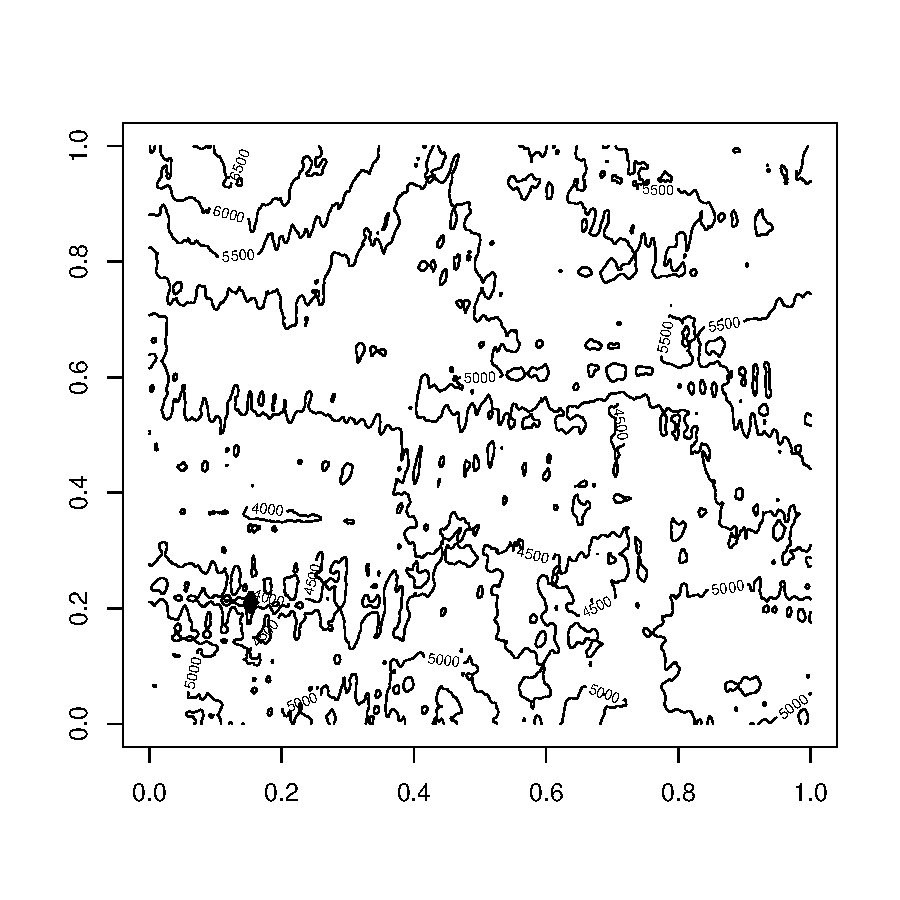
\includegraphics{template_matching-004}
\caption{Superfície de contorno para placa 1 e p igual a 1.}
\label{placa1p1}
\end{figure}

\begin{Schunk}
\begin{Sinput}
> result_p1 <- which(d_list[[1]][[1]] == min(d_list[[1]][[1]]), arr.ind = TRUE)
> print(c("O valor mínimo é: ",  min(d_list[[1]][[1]])))
\end{Sinput}
\begin{Soutput}
[1] "O valor mínimo é: " "99.8352941176471"  
\end{Soutput}
\begin{Sinput}
> print(c(" Está no ponto: ",
+         which(d_list[[1]][[1]] == min(d_list[[1]][[1]]), arr.ind = TRUE)))
\end{Sinput}
\begin{Soutput}
[1] " Está no ponto: " "87"               "71"              
\end{Soutput}
\begin{Sinput}
> print(c("Razão entre a média e o mínimo", 
+         mean(d_list[[1]][[1]])/ min(d_list[[1]][[1]])))
\end{Sinput}
\begin{Soutput}
[1] "Razão entre a média e o mínimo" "49.5964174587175"              
\end{Soutput}
\end{Schunk}

\begin{figure}
\centering
\begin{Schunk}
\begin{Sinput}
> plot_image(Im, result_p1 = result_p1, cor = cor)
\end{Sinput}
\end{Schunk}
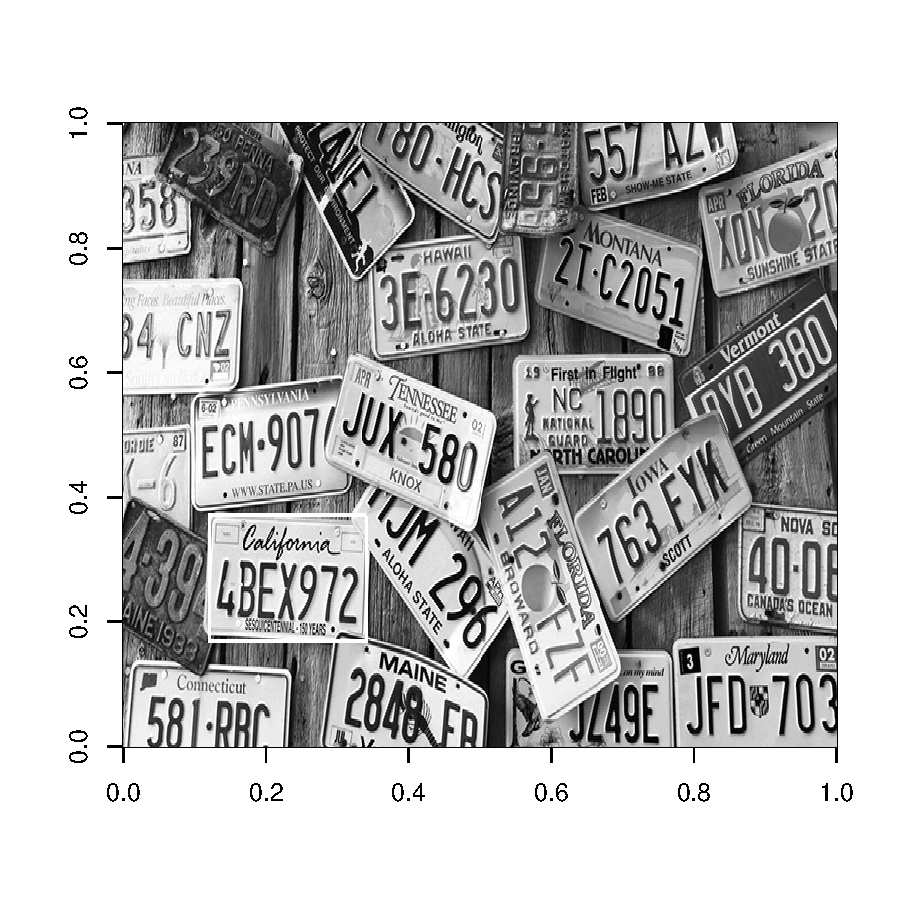
\includegraphics{template_matching-006}
\caption{Imagem com a placa 1 selecionada no conjunto de placas,para p igual a 1.}
\label{placa1selecionada}
\end{figure}

% Figura 2
\begin{figure}
 \centering
\begin{Schunk}
\begin{Sinput}
>  contour(d_list[[1]][[2]])
\end{Sinput}
\end{Schunk}
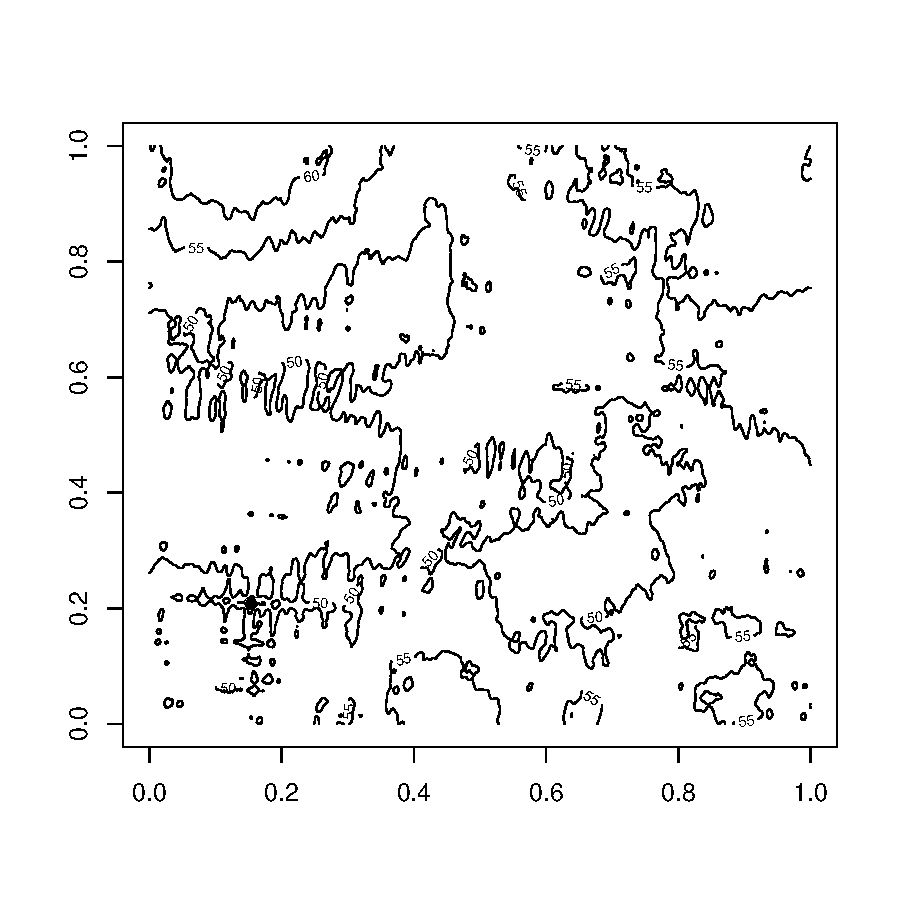
\includegraphics{template_matching-007}
 \caption{Superfície de contorno para placa 1 e p igual a 2.}
 \label{placa1p2}
\end{figure}
\begin{Schunk}
\begin{Sinput}
>  result_p2 <- which(d_list[[1]][[2]] == min(d_list[[1]][[2]]), arr.ind = TRUE)
>  print(c("O valor mínimo é: ",  min(d_list[[1]][[2]])))
\end{Sinput}
\begin{Soutput}
[1] "O valor mínimo é: " "1.1379984046952"   
\end{Soutput}
\begin{Sinput}
>  print(c(" Está no ponto: ",
+          which(d_list[[1]][[2]] == min(d_list[[1]][[2]]), arr.ind = TRUE)))
\end{Sinput}
\begin{Soutput}
[1] " Está no ponto: " "87"               "71"              
\end{Soutput}
\begin{Sinput}
> print(c("Razão entre a média e o mínimo", 
+         mean(d_list[[1]][[2]])/ min(d_list[[1]][[2]])))
\end{Sinput}
\begin{Soutput}
[1] "Razão entre a média e o mínimo" "45.8000607641388"              
\end{Soutput}
\end{Schunk}
\begin{figure}
\centering
\begin{Schunk}
\begin{Sinput}
> plot_image(Im, result_p1 = result_p2, cor = cor)
\end{Sinput}
\end{Schunk}
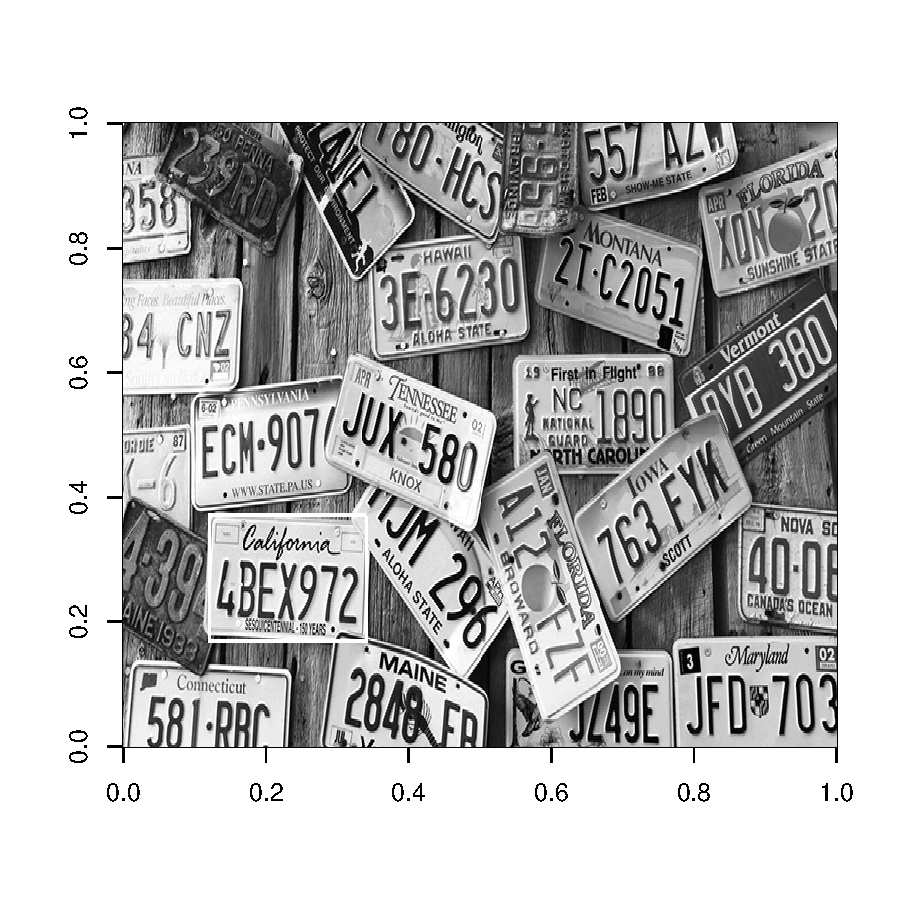
\includegraphics{template_matching-009}
\caption{Imagem com a placa 1 selecionada no conjunto de placas,para p igual a 2.}
\label{placa1selecionada}
\end{figure}

\begin{figure}
\centering
\begin{Schunk}
\begin{Sinput}
> contour(d_list[[1]][[3]])
\end{Sinput}
\end{Schunk}
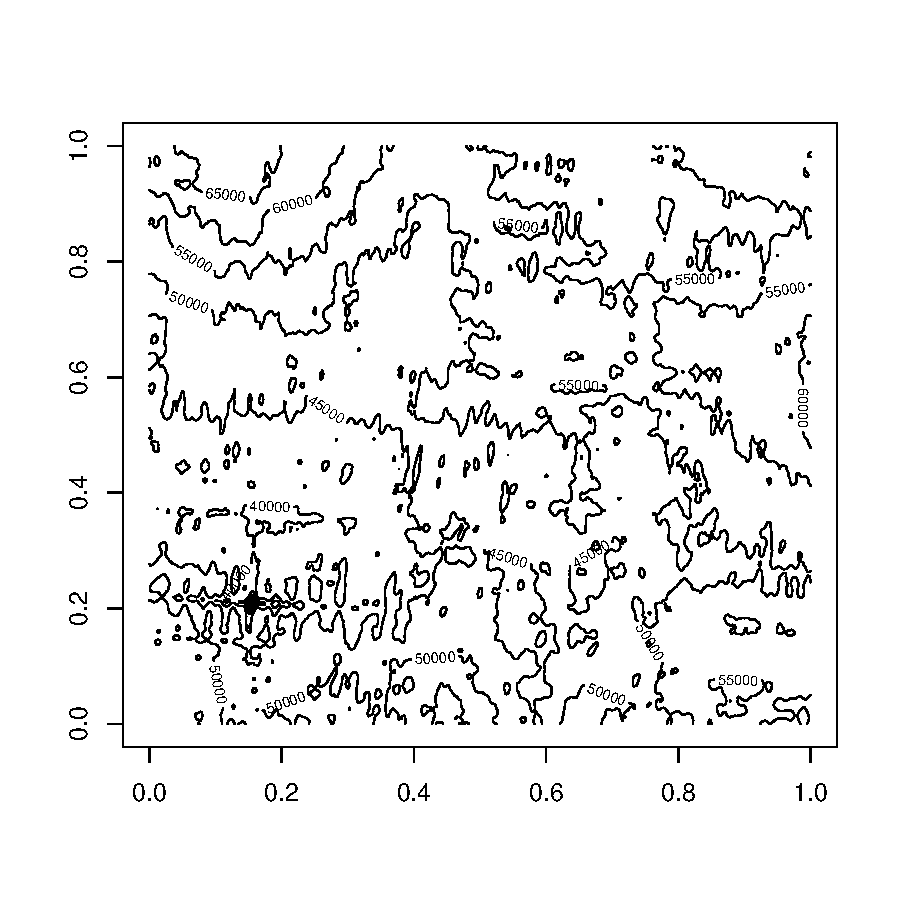
\includegraphics{template_matching-010}
\caption{Superfície de contorno para placa 1 e p igual a 0.8.}
\label{placa1p08}
\end{figure}
\begin{Schunk}
\begin{Sinput}
> result_p08 <- which(d_list[[1]][[3]] == min(d_list[[1]][[3]]), arr.ind = TRUE)
> print(c("O valor mínimo é: ",  min(d_list[[1]][[3]])))
\end{Sinput}
\begin{Soutput}
[1] "O valor mínimo é: " "985.613954530948"  
\end{Soutput}
\begin{Sinput}
> print(c(" Está no ponto: ",
+         which(d_list[[1]][[3]] == min(d_list[[1]][[3]]), arr.ind = TRUE)))
\end{Sinput}
\begin{Soutput}
[1] " Está no ponto: " "87"               "71"              
\end{Soutput}
\begin{Sinput}
> print(c("Razão entre a média e o mínimo", 
+         mean(d_list[[1]][[3]])/ min(d_list[[1]][[3]])))
\end{Sinput}
\begin{Soutput}
[1] "Razão entre a média e o mínimo" "51.1572353658518"              
\end{Soutput}
\end{Schunk}
\begin{figure}
\centering
\begin{Schunk}
\begin{Sinput}
> plot_image(Im, result_p1 = result_p08, cor = cor)
\end{Sinput}
\end{Schunk}
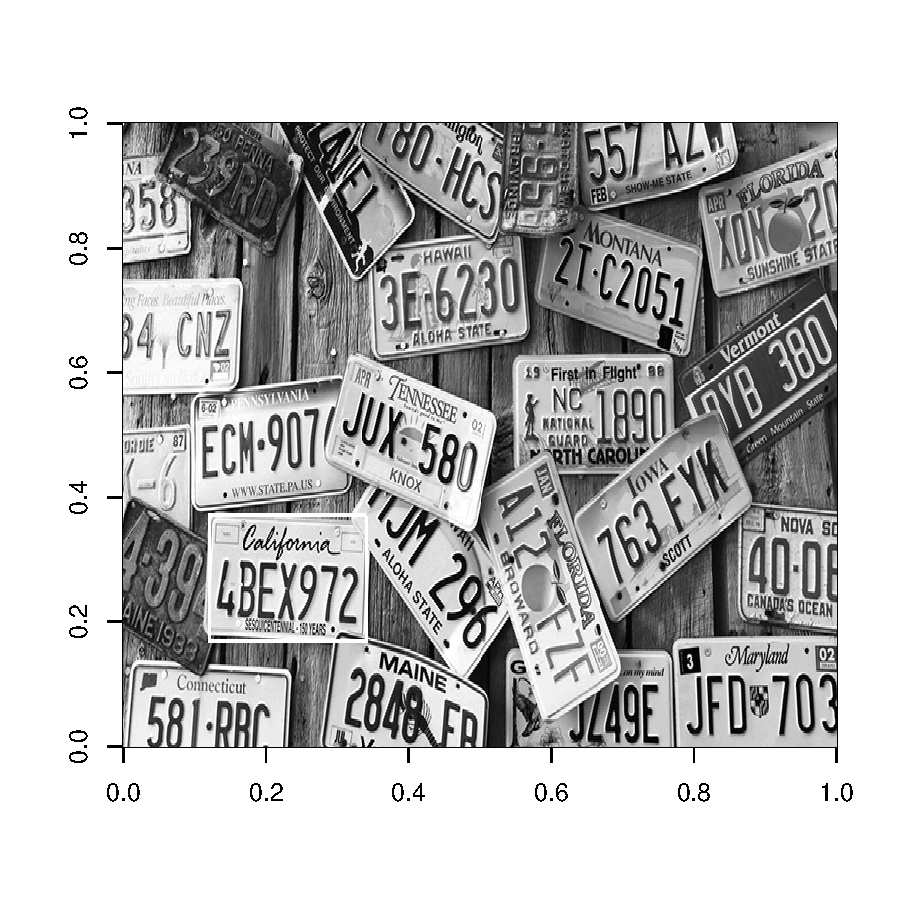
\includegraphics{template_matching-012}
\caption{Imagem com a placa 1 selecionada no conjunto de placas,para p igual a 0.8}
\label{placa1selecionada}
\end{figure}
\begin{figure}
\centering
\begin{Schunk}
\begin{Sinput}
> contour(d_list[[1]][[4]])
\end{Sinput}
\end{Schunk}
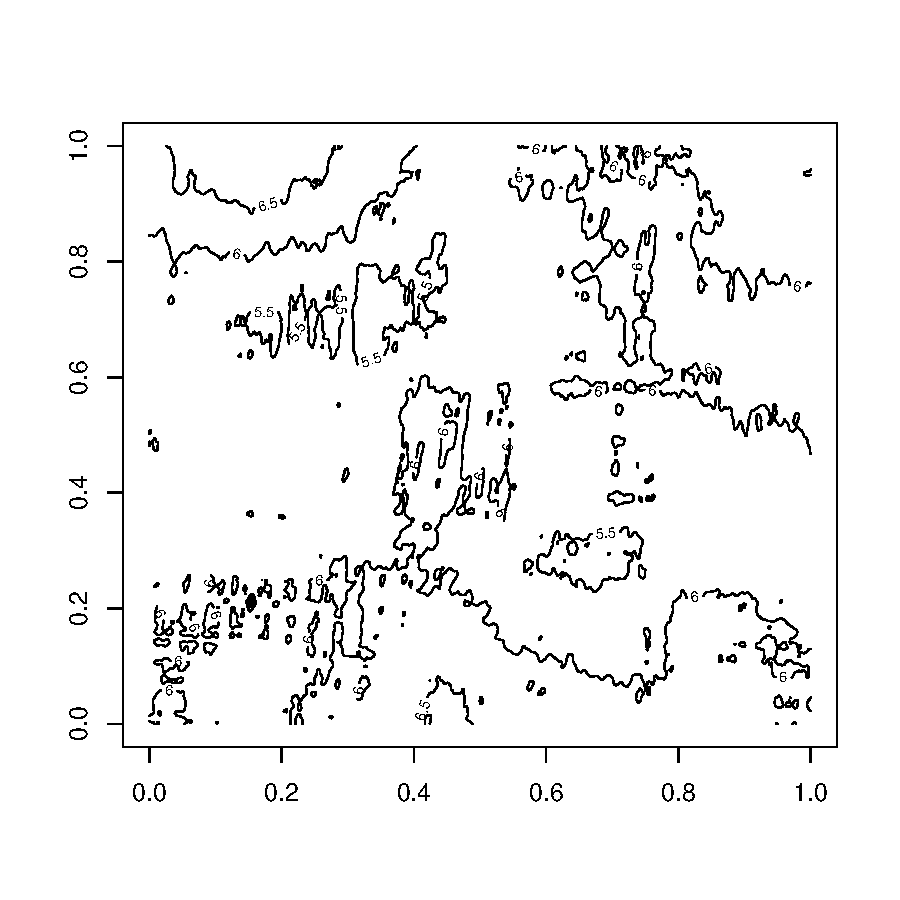
\includegraphics{template_matching-013}
\caption{Superfície de contorno para placa 1 e p igual a 4.}
\label{placa1p4}
\end{figure}
\begin{Schunk}
\begin{Sinput}
> result_p4 <- which(d_list[[1]][[4]] == min(d_list[[1]][[4]]), arr.ind = TRUE)
> print(c("O valor mínimo é: ",  min(d_list[[1]][[4]])))
\end{Sinput}
\begin{Soutput}
[1] "O valor mínimo é: " "0.148135761890773" 
\end{Soutput}
\begin{Sinput}
> print(c(" Está no ponto: ",
+         which(d_list[[1]][[4]] == min(d_list[[1]][[4]]), arr.ind = TRUE)))
\end{Sinput}
\begin{Soutput}
[1] " Está no ponto: " "87"               "71"              
\end{Soutput}
\begin{Sinput}
> print(c("Razão entre a média e o mínimo", 
+         mean(d_list[[1]][[4]])/ min(d_list[[1]][[4]])))
\end{Sinput}
\begin{Soutput}
[1] "Razão entre a média e o mínimo" "39.8790442311116"              
\end{Soutput}
\end{Schunk}
\begin{figure}
\centering
\begin{Schunk}
\begin{Sinput}
> plot_image(Im, result_p1 = result_p4, cor = cor)
\end{Sinput}
\end{Schunk}
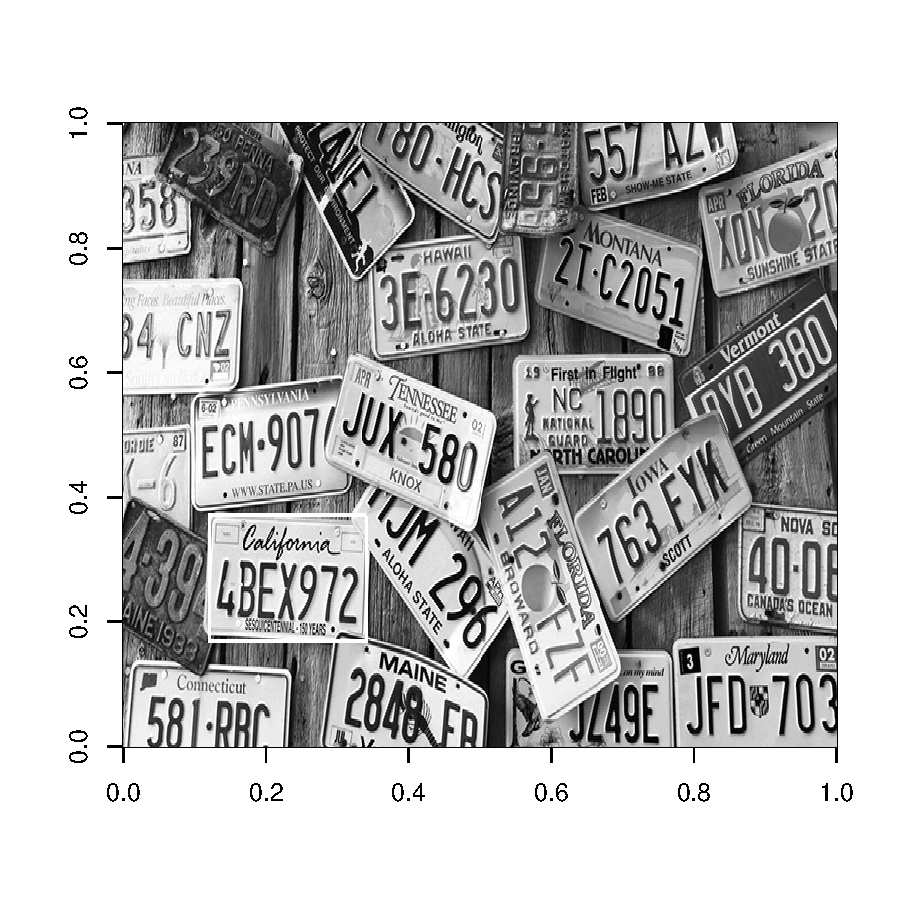
\includegraphics{template_matching-015}
\caption{Imagem com a placa 1 selecionada no conjunto de placas,para p igual a 4.}
\label{placa1selecionada}
\end{figure}


\begin{Schunk}
\begin{Sinput}
> p <- c(1, 2, 0.8, 4)
> results <- find_board(p, p2, Im)
> min_dist_1 <- results[1]
> d_list <- results[2]
\end{Sinput}
\end{Schunk}

\begin{figure}
\centering
\begin{Schunk}
\begin{Sinput}
> contour(d_list[[1]][[1]])
\end{Sinput}
\end{Schunk}
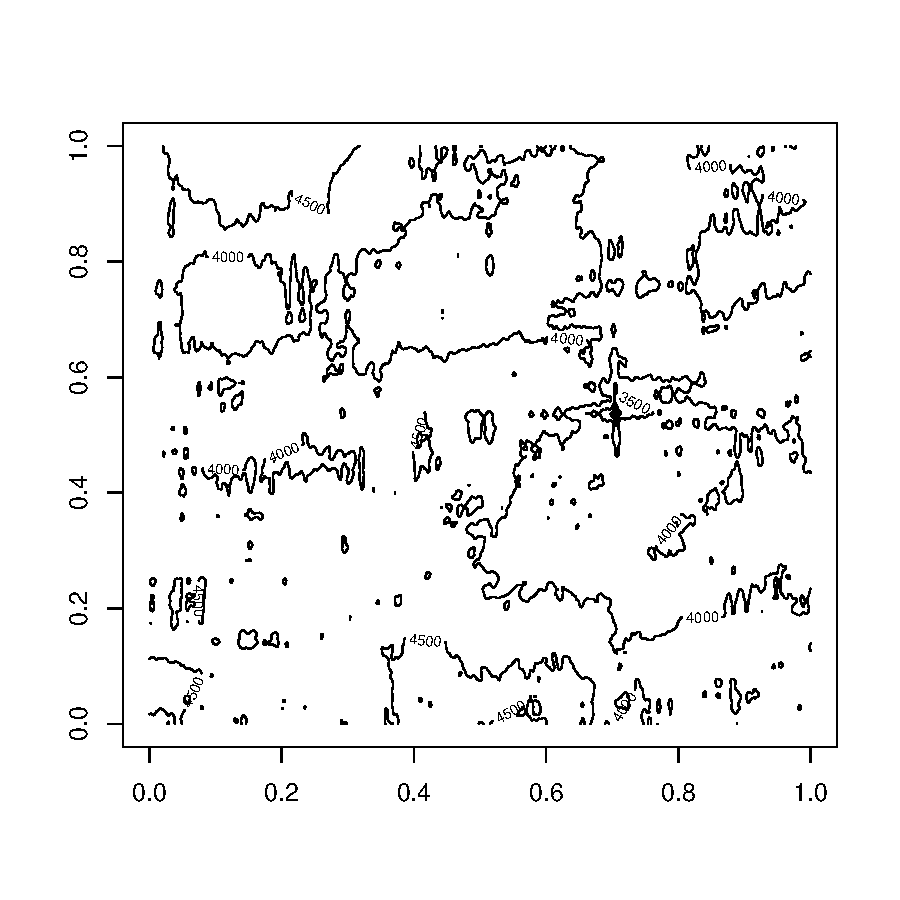
\includegraphics{template_matching-017}
\caption{Superfície de contorno para placa 2 e p igual a 1.}
\label{placa1p1}
\end{figure}

\begin{Schunk}
\begin{Sinput}
> result_p1 <- which(d_list[[1]][[1]] == min(d_list[[1]][[1]]), arr.ind = TRUE)
> print(c("O valor mínimo é: ",  min(d_list[[1]][[1]])))
\end{Sinput}
\begin{Soutput}
[1] "O valor mínimo é: " "117.76862745098"   
\end{Soutput}
\begin{Sinput}
> print(c(" Está no ponto: ",
+         which(d_list[[1]][[1]] == min(d_list[[1]][[1]]), arr.ind = TRUE)))
\end{Sinput}
\begin{Soutput}
[1] " Está no ponto: " "394"              "183"             
\end{Soutput}
\begin{Sinput}
> print(c("Razão entre a média e o mínimo", 
+         mean(d_list[[1]][[1]])/ min(d_list[[1]][[1]])))
\end{Sinput}
\begin{Soutput}
[1] "Razão entre a média e o mínimo" "34.928060556941"               
\end{Soutput}
\end{Schunk}

\begin{figure}
\centering
\begin{Schunk}
\begin{Sinput}
> plot_image(Im, result_p1 = result_p1, cor = cor)
\end{Sinput}
\end{Schunk}
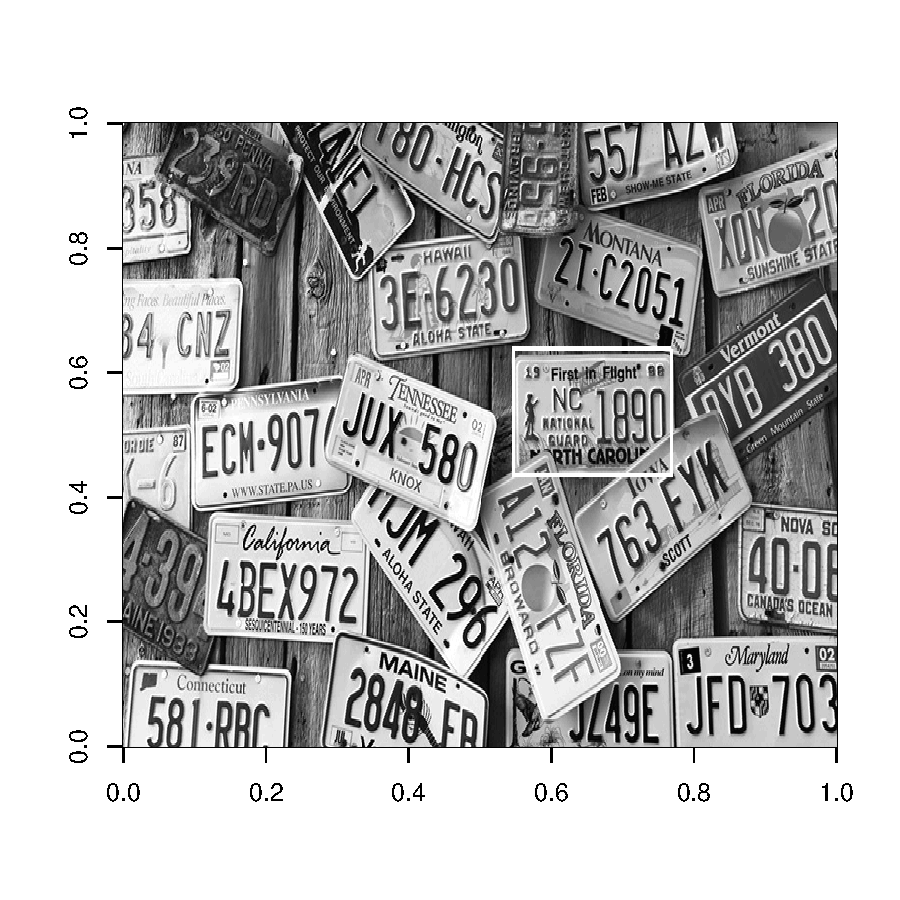
\includegraphics{template_matching-019}
\caption{Imagem com a placa 2 selecionada no conjunto de placas,para p igual a 1.}
\label{placa1selecionada}
\end{figure}

% Figura 2
\begin{figure}
 \centering
\begin{Schunk}
\begin{Sinput}
>  contour(d_list[[1]][[2]])
\end{Sinput}
\end{Schunk}
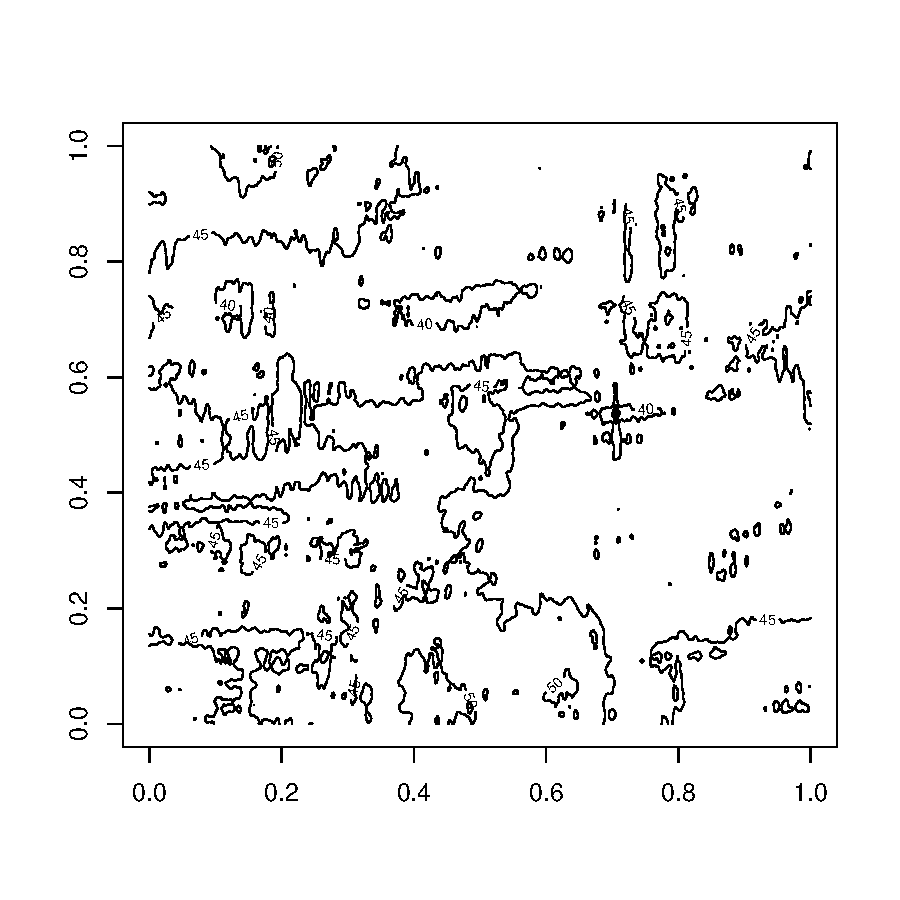
\includegraphics{template_matching-020}
 \caption{Superfície de contorno para placa 2 e p igual a 2.}
 \label{placa1p2}
\end{figure}
\begin{Schunk}
\begin{Sinput}
>  result_p2 <- which(d_list[[1]][[2]] == min(d_list[[1]][[2]]), arr.ind = TRUE)
>  print(c("O valor mínimo é: ",  min(d_list[[1]][[2]])))
\end{Sinput}
\begin{Soutput}
[1] "O valor mínimo é: " "1.33881801577141"  
\end{Soutput}
\begin{Sinput}
>  print(c(" Está no ponto: ",
+          which(d_list[[1]][[2]] == min(d_list[[1]][[2]]), arr.ind = TRUE)))
\end{Sinput}
\begin{Soutput}
[1] " Está no ponto: " "394"              "183"             
\end{Soutput}
\begin{Sinput}
>  print(c("Razão entre a média e o mínimo", 
+         mean(d_list[[1]][[2]])/ min(d_list[[1]][[2]])))
\end{Sinput}
\begin{Soutput}
[1] "Razão entre a média e o mínimo" "33.1503557828145"              
\end{Soutput}
\end{Schunk}
\begin{figure}
\centering
\begin{Schunk}
\begin{Sinput}
> plot_image(Im, result_p1 = result_p2, cor = cor)
\end{Sinput}
\end{Schunk}
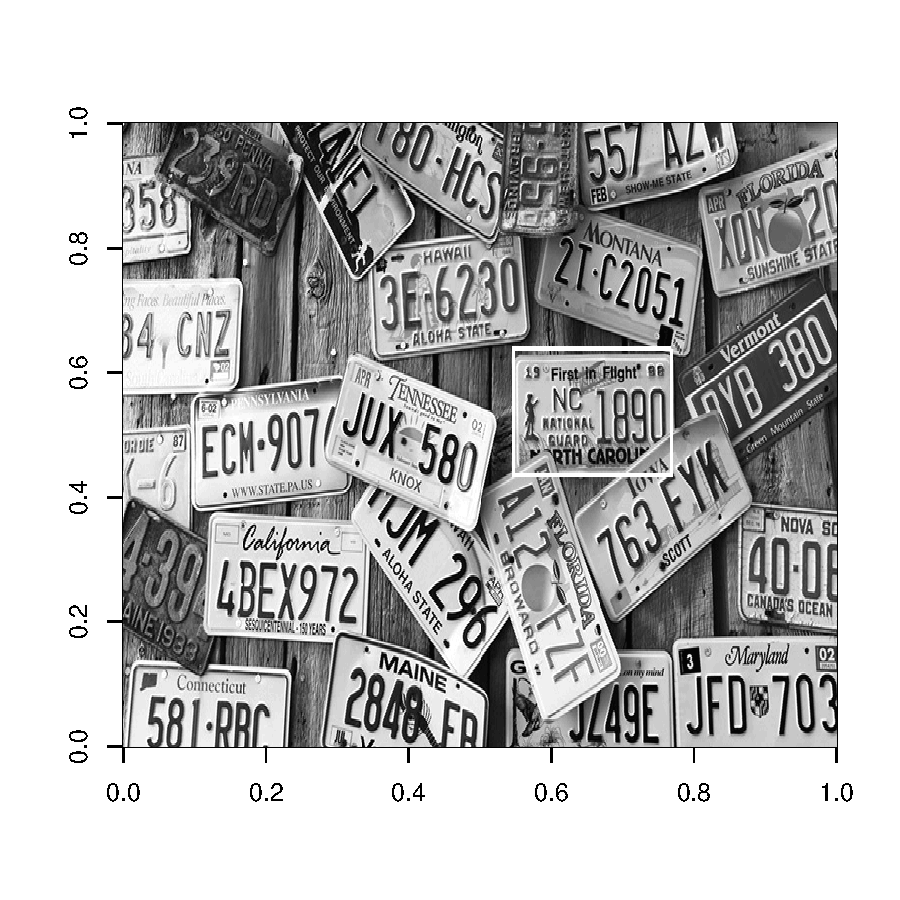
\includegraphics{template_matching-022}
\caption{Imagem com a placa 2 selecionada no conjunto de placas,para p igual a 2.}
\label{placa1selecionada}
\end{figure}

\begin{figure}
\centering
\begin{Schunk}
\begin{Sinput}
> contour(d_list[[1]][[3]])
\end{Sinput}
\end{Schunk}
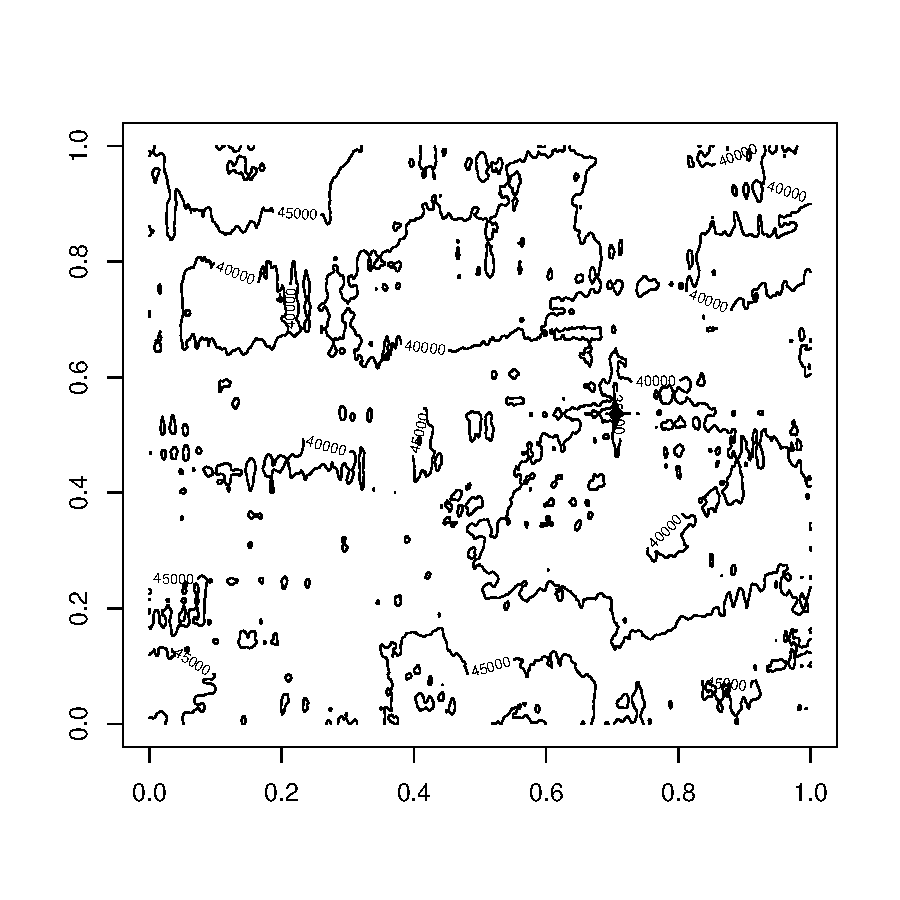
\includegraphics{template_matching-023}
\caption{Superfície de contorno para placa 2 e p igual a 0.8.}
\label{placa2p08}
\end{figure}
\begin{Schunk}
\begin{Sinput}
> result_p08 <- which(d_list[[1]][[3]] == min(d_list[[1]][[3]]), arr.ind = TRUE)
> print(c("O valor mínimo é: ",  min(d_list[[1]][[3]])))
\end{Sinput}
\begin{Soutput}
[1] "O valor mínimo é: " "1160.02884879164"  
\end{Soutput}
\begin{Sinput}
> print(c(" Está no ponto: ",
+         which(d_list[[1]][[3]] == min(d_list[[1]][[3]]), arr.ind = TRUE)))
\end{Sinput}
\begin{Soutput}
[1] " Está no ponto: " "394"              "183"             
\end{Soutput}
\begin{Sinput}
> print(c("Razão entre a média e o mínimo", 
+         mean(d_list[[1]][[3]])/ min(d_list[[1]][[3]])))
\end{Sinput}
\begin{Soutput}
[1] "Razão entre a média e o mínimo" "35.7278894967374"              
\end{Soutput}
\end{Schunk}
\begin{figure}
\centering
\begin{Schunk}
\begin{Sinput}
> plot_image(Im, result_p1 = result_p08, cor = cor)
\end{Sinput}
\end{Schunk}
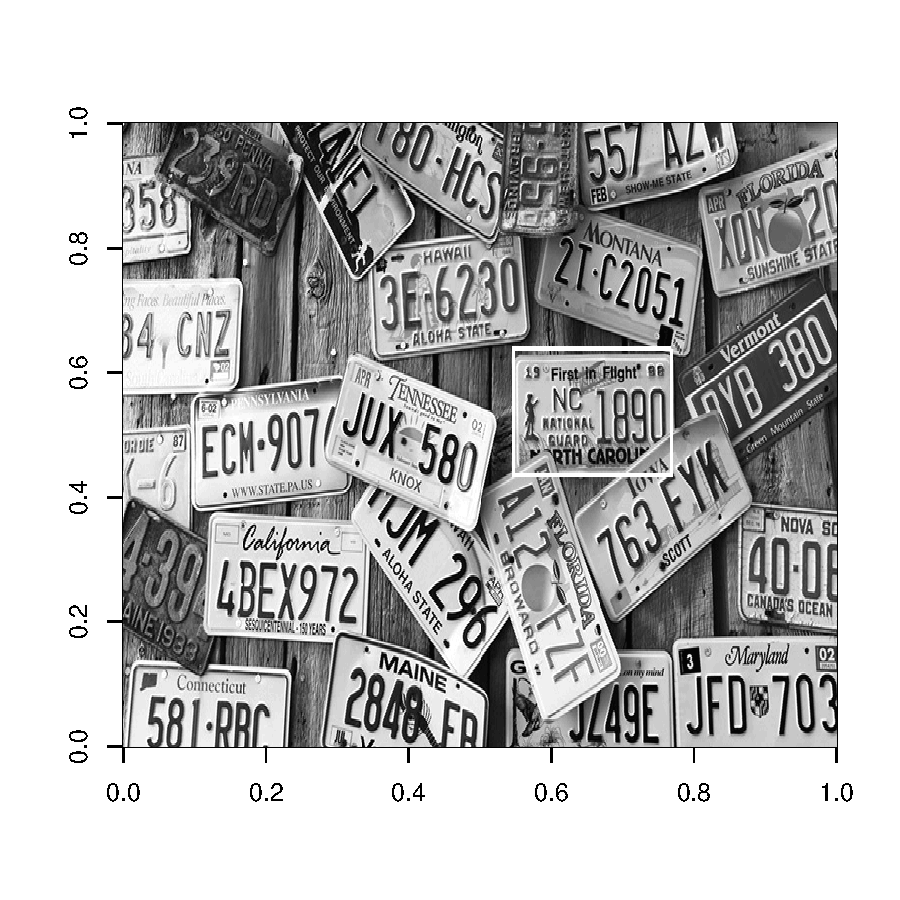
\includegraphics{template_matching-025}
\caption{Imagem com a placa 2 selecionada no conjunto de placas,para p igual a 0.8}
\label{placa1selecionada}
\end{figure}
\begin{figure}
\centering
\begin{Schunk}
\begin{Sinput}
> contour(d_list[[1]][[4]])
\end{Sinput}
\end{Schunk}
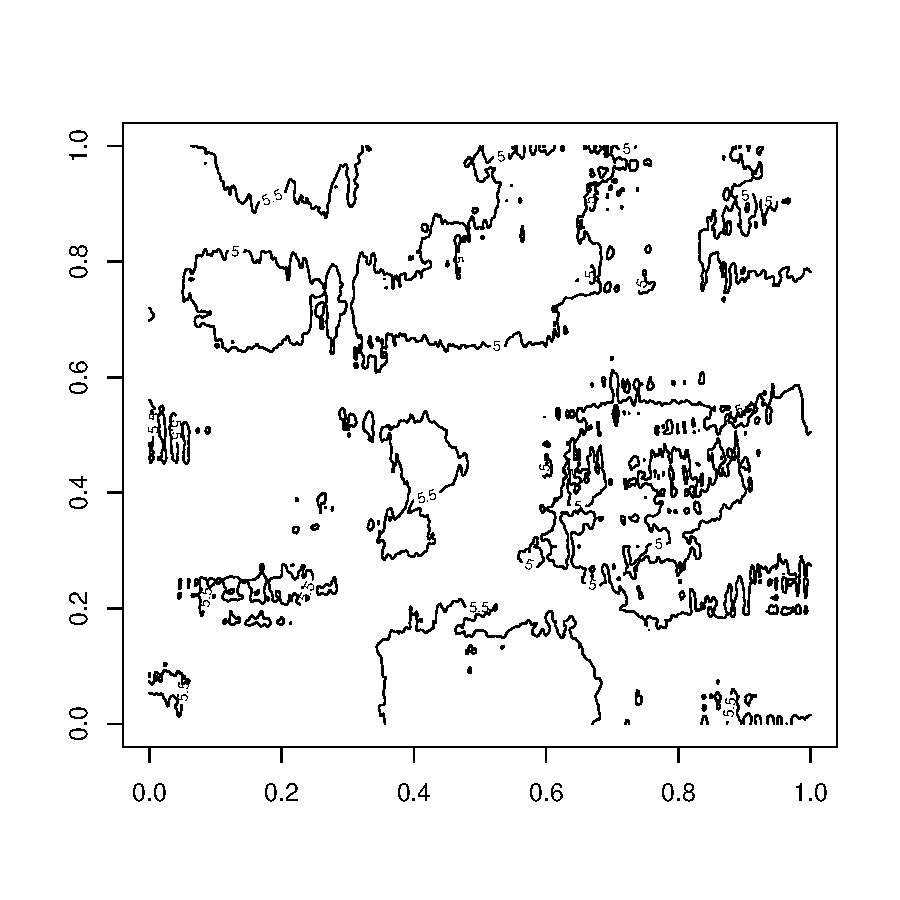
\includegraphics{template_matching-026}
\caption{Superfície de contorno para placa 2 e p igual a 4.}
\label{placa2p4}
\end{figure}
\begin{Schunk}
\begin{Sinput}
> result_p4 <- which(d_list[[1]][[4]] == min(d_list[[1]][[4]]), arr.ind = TRUE)
> print(c("O valor mínimo é: ",  min(d_list[[1]][[4]])))
\end{Sinput}
\begin{Soutput}
[1] "O valor mínimo é: " "0.168886345419138" 
\end{Soutput}
\begin{Sinput}
> print(c(" Está no ponto: ",
+         which(d_list[[1]][[4]] == min(d_list[[1]][[4]]), arr.ind = TRUE)))
\end{Sinput}
\begin{Soutput}
[1] " Está no ponto: " "394"              "183"             
\end{Soutput}
\begin{Sinput}
> print(c("Razão entre a média e o mínimo", 
+         mean(d_list[[1]][[4]])/ min(d_list[[1]][[4]])))
\end{Sinput}
\begin{Soutput}
[1] "Razão entre a média e o mínimo" "30.7532181923793"              
\end{Soutput}
\end{Schunk}
\begin{figure}
\centering
\begin{Schunk}
\begin{Sinput}
> plot_image(Im, result_p1 = result_p4, cor = cor)
\end{Sinput}
\end{Schunk}
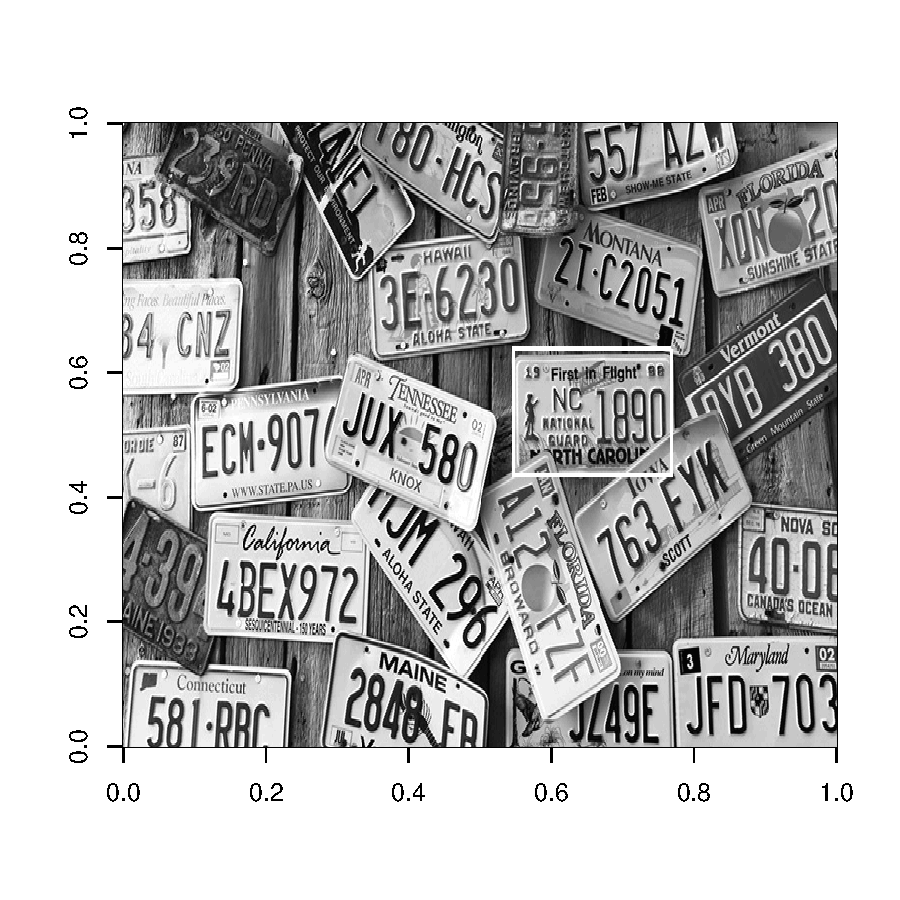
\includegraphics{template_matching-028}
\caption{Imagem com a placa 2 selecionada no conjunto de placas,para p igual a 4.}
\label{placa2selecionada}
\end{figure}

\section{Discussão}
    \par A priori, pensei que o algoritmo que tivesse a menor distância seria o melhor. No entanto, quando queremos discenir algo, é melhor comparar o quanto o valores de distância se diferem uns dos outros ao longo da imagem. Isso é obtido ao fazer a razão entre a média e o mínimo. Dessa forma, o maior valor encontrado na razão corresponderá o melhor valor de p.  Como podemos ver os melhore valores encontrados foram p igual 0.8 para as duas placas. Mas note que todos conseguiram de forma satisfatória encontra a placa. 
    
    \par Outro fator importante é que quando analisamos os contornos para os melhores valores de p, figuras \ref{placa1p08} e \ref{placa2p08}, podemos ver que há uma grande diferença entre o mínimo e as linhas de relevo mais próximas.
    
    \par É valido comentar que o algoritmo se mostrou ineficiente em termos de tempo de execução. Por esse motivo, não foi possível expandir a análise para outros valores de p, já que levaria muito tempo para executar todo o código.

    \par Pelos motivos supracitados, pode-se afirmar que os objetivos do experimento foram atingidos, uma vez que foi possível comparar métricas de distância e construir um algoritmo de Template Matching capaz de encontrar as duas placas de interesse.
%%%%%%%%%%%%%%%%%%%%%%%%%%%%%%%%%%%%%%%%%%%%%%%%%%%%%%%%%%%%%%%%%%%%%%%%%%%%%%%%%%%%%%%%%

%%%%%%%%%%%%%%%%%%%%%%%%%%%%%%%%%%%%%%%%%%%%%%%%%%%%%%%%%%%%%%%%%%%%%%%%%%%%%%%%%%%%%%%%%


\end{document}
